\section{Garbage Collection}
\begin{definition}[Garbage]
    Heap-allocated records that are not reachable by any chain of pointers from program variables are garbage.
\end{definition}

不存在一个通用程序能算出每一个变量是否活跃, 所以使用一个保守的近似: 要求编译器保证所有活跃记录是可达的(reachable), 并最小化可达的不活跃记录. 

\subsection{Mark-and-sweep Collection}
程序变量与堆分配记录可以构成一张有向图. 变量就是图的一系列根.

\begin{definition}[reachable]
    A node $n$ is reachable if there is a path of directed edges $r \to\cdots \to  n$ starting at some root $r$.
\end{definition}

算法原理:
\begin{enumerate}
    \item 标记: 使用 DFS 标记所有可达节点
    \item 清扫: 未被标记的节点都是垃圾, 从头到尾扫描堆内存, 将未标记的节点加到空闲表(freelist)中, 同时清除已标记节点的标记. 
\end{enumerate}

\subsubsection{Cost of garbage collection}
假设大小为 $H$ 个字的堆中, 有 $R$ 个字可达, 则一次垃圾回收的代价是 $c_1R+c_2H$, 其中 $c_1, c_2$ 为常数. 

最终每个垃圾的均摊回收代价是 
\begin{align*}
    \frac{c_1R+c_2H}{H-R}
\end{align*}
若 $\frac{R}{H}>0.5$, 回收器应该向 OS 申请更大的内存, 以增大 $H$.

\subsubsection{Optimization}
对算法的空间与时间常数进行优化. 

\begin{itemize}
    \item 使用显式的栈(explicit stack): 将 DFS 的递归改写为循环. 因为递归的 DFS 其运行时的栈可能超过总的堆大小, 所以用显式的栈代替使用堆.
    \item 指针翻转(Pointer reversal): 压栈时使用 $x.f_i$ 指向其父节点, 弹栈时用  $x.f_i$ 的值找到父节点, 再恢复其原本的值, 这样连显示的栈都不需要. 只需要额外的 $done$ 数组作为 $x$ 子域的下标.
\end{itemize}

DFS 中, $x$ 是当前节点, $t$ 是父节点, $y$ 是子节点, $done[x]$ 用于索引 $x.f_{done[x]}$ 作为下一个子域. 

% \begin{figure}[H]
%     \centering
%     \includegraphics[width=0.618\linewidth]{pic/CP13/Depth-first search}
%     \caption{Mark-and-sweep's DFS}
% \end{figure}

\subsubsection{An Array of Freelists} 
$freelists$ 使用空闲域的大小作为索引, 存储邻接链表, 方便之后使用. 比如想要大小为 $i$ 的域, 把 $freelists[i]$ 的头取出即可. 也可以取出 $freelists[j](j>i)$, 然后把剩下的空闲域插入 $freelists[j-i]$.

\subsubsection{Fragment}
\begin{itemize}
    \item 外部碎片(external fragmentation): 想分配一个 $n$ 大小的空间, 但是空闲空间均小于 $n$.
    \item 内部碎片(internal fragmentation): 实际使用大小为 $n$ , 却分 配 了 大 小 为 $K(K>n)$ 的 空 间, 未使用的空间在记录内而不是在空闲表中.
\end{itemize}

\subsection{Reference Counts}
算法原理: 记住每个记录有多少指针指向其, 计数和每个记录储存在一起. 

\begin{itemize}
    \item 当 $p$ 写入 $x.f_i$ 时, $p$ 的引用数要增加, $x.f_i$ 之前内容的引用数要减少. 
    \item 若 $r$ 的引用数为 0, 将 $r$ 加入到 $freelist$ 中, 并减少 $r$ 指向的其他记录的引用数. 
\end{itemize}

有一个改进是在将 $r$ 从 $freelist$ 中删除时,再递归地减少 $r.f_i$ 的计数:
\begin{enumerate}
    \item 能将递归减少的动作分解为较短的操作, 使程序的运行更加平滑(对对交互式程序或实时程序好)
    \item 递归减少动作只需要在分配 $r$ 时进行. 
\end{enumerate}

但有两个大问题:
\begin{enumerate}
    \item 无法回收成环的垃圾.
    \item 增加引用计数所需的操作代价很大.
\end{enumerate}

解决``环''的办法:
\begin{enumerate}
    \item 让程序员手动断开所有循环引用, 这比手动管理内存要简单, 但也并不优雅.
    \item 将标记清理(快速, 无中断地回收)和引用计数(回收环)相结合.
\end{enumerate}

引用计数的缺点大于优点, 所以极少使用. 

\subsection{Copying Collection}
\begin{enumerate}
    \item 将堆分为两块区 域 from-space 和 to-space; 当 前 的 内 存 放 到 from-space 中 
    \item 在 to-space 构造一个同构的副本, 副本空间利用上更紧凑: 占据连续的不含碎片的储存单元
    \item from-space 和 to-space 互换, 然后抛弃 from-space. 
\end{enumerate}

\begin{figure}[H]
    \centering
    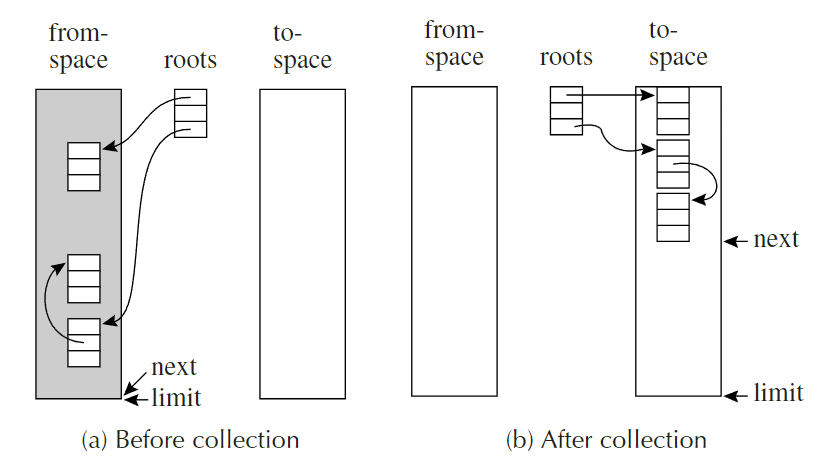
\includegraphics[width=0.84\linewidth]{pic/CP13/Copying collection}
    \caption{Copying collection}
\end{figure}

算法流程:
\begin{enumerate}
    \item 回收初始化: 初始化指针 next 指向 to-space 的开始. 每当 from-space 发现一个可达记录, 便把它复制到 to-space 的 next 所指位置, 同时使 next 增 加 该 记 录 的 大 小. 
    \item 转递(forwarding): 使一个指向 from-space 的指针 $p$ 转而指向 to-space. 有三种情况:
    \begin{enumerate}
        \item 若 $p$ 指向的 from-space 已经被复制, 则 $p.f_1$ 是一个特殊的转递指针(forwarding pointer)指向了副本所在. 因为只有这种指针指向了 to-space, 可以很容易地分辨. 
        \item 若 $p$ 指向的 from-space 未被复制, 则将其复制到 next 所在位置, 然后将 $p.f_1$ 变为转递指针. 因为其已经被复制了, 所以可以覆写 $f_1$.
        \item 若 $p$ 不是指针或指向了 from-space 之外, 不做任何事. 
    \end{enumerate}
\end{enumerate}

\subsubsection{Cheney's algorithm}
使用 BFS 遍历可达数据. 

\begin{figure}[H]
    \centering
    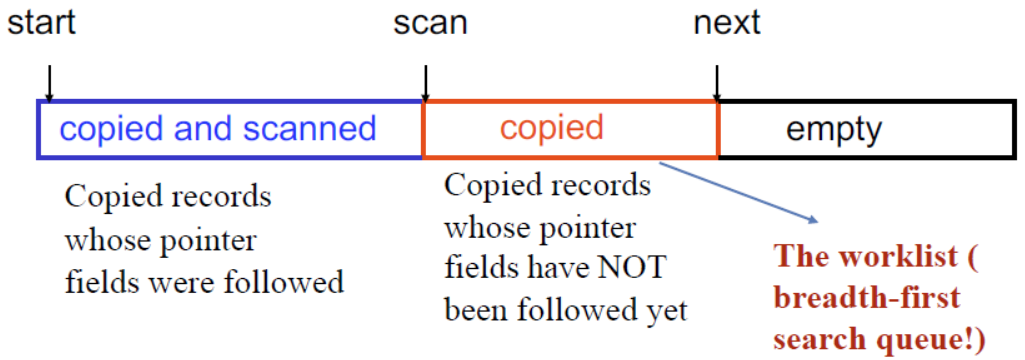
\includegraphics[width=0.84\linewidth]{pic/CP13/Cheney's algorithm}
    \caption{Cheney's algorithm}
\end{figure}

\begin{itemize}
    \item 在 to-space 上, 位于 scan 与 next 之间包含了已经被复制到 to-sapce, 但是其子域还没有转递的记录, 他们的子域仍指向着 from-space. 
    \item 在 scan 之前包含了被复制且被转递的记录, 其中所有指针都指向 to-space.
\end{itemize}

但其空间局部性不好, $x$ 中的指针 $x.f_i$ 指向的对象可能地址离 $x$ 很远, 这导致无法很好的利用虚拟内存, 也会造成许多 cache misses.  DFS 的局部性很好, 但需要各种复杂的常数优化. 所以结合 BFS 与 DFS, 用 BFS 寻找需要复制的记录, 复制时使用 DFS 复制. 


\subsubsection{Cost of garbage collection}
假设大小为 $H$ 个字的堆中, 有 $R$ 个字可达, 因为 $H$ 被分为了两部分, 所以只需要回收 $\frac{H}{2}-R$ 的垃圾. 对每个垃圾的均摊回收代价为
\begin{align*}
    \frac{c_3R}{\frac{H}{2}-R}
\end{align*}
其中 $c_3$ 是常数. 


\subsection{Interface to the Compiler}
\subsubsection{Fast Allocation}
使用复制回收(copying collection)的方式回收垃圾, 以便分配空间是一个连续的空闲区域. 区 域 的 末 端 是 limit, next 指向下一个空闲单元.


分配大小为 $N$ 的记录的步骤如下: 
\begin{enumerate}
    \item 调用分配函数
    \item 若 $next+N<limit$ 则继续, 否则调用垃圾回收.
    \item 将 $next$ 复制到 $result$
    \item 清理 $M[next], M[next+1],\dots,M[next+N-1]$
    \item $next\leftarrow next+N$
    \item 从分配函数返回. 
    \begin{enumerate}
        \item 将 $result$ 赋值到计算上有用的地方.
        \item 将要 用 到 的 值 储 存 到 该 记 录 
    \end{enumerate}
\end{enumerate}

使用内联展开(inline expanding, 将函数调用替换为函数本体)可以省略 1) 和 6); 与 a. 结合可以消除 3); b. 也可以消除 4); 2), 5) 不能被消除. 但若是多个分配可以被合并优化. 至此, 分配就减少到了大约4条指令. 

\subsubsection{Describing Data Layouts}
垃圾回收器需要对任意数据类型进行操作, 所以需要确定每条记录的子域类型及数量. 简单的方法是用每个对象指针的第一个字指向一个描述记录(descripter record), 其包含对象总大小, 以及每个域指针的位置. 

垃圾回收器需要知道哪些内存地址是指针, 才能正确地跟踪对象间的引用关系, 避免错误地回收正在使用的对象. 所以编译器需要生成指针映射(pointer map)来描述程序运行过程中每个时刻哪些位置存储着指针. 

具体步骤:
\begin{enumerate}
    \item 识别指针: 编译器需要识别出所有可能包含指针的变量, 包括堆记录, 临时变量和局部变量, 无论它们存储在寄存器还是活动记录(activation record)中. 
    \item 指针映射的时机: 由于活跃指针的集合在每条指令执行后都可能发生变化, 所以为每条指令都生成指针映射是不现实的. 因此, 编译器只在垃圾回收可能开始的点生成指针映射, 这些点包括:
    \begin{itemize}
        \item 调用 alloc 函数的地方, 因为分配新内存可能会触发垃圾回收. 
        \item 每个函数调用的地方, 因为被调用的函数可能直接或间接地调用 alloc 函数. 
    \end{itemize}
    \item 指针映射的组织: 指针映射使用函数返回地址作为键, 因为返回地址是垃圾回收器在下一个活动记录中看到的内容. 每个返回地址对应一个活跃指针集合, 描述了在该返回地址处哪些寄存器或栈帧位置存储着指针. 
    \item 垃圾回收过程: 垃圾回收器从栈顶开始向下扫描, 逐帧查找活跃指针. 
    \begin{itemize}
        \item 每个返回地址都指向一个指针映射条目, 该条目描述了下一帧的信息. 
        \item 在每一帧中, 垃圾回收器根据指针映射标记/转递(取决于垃圾回收方式)该帧中的所有活跃指针. 
    \end{itemize}
    \item callee-save 寄存器: 对于 callee-save 寄存器, 需要特殊处理. 
    \subitem 例如, 函数 $f$ 调用 $g$, $g$ 调用 $h$. 函数 $h$ 知道它将一些 callee-save 寄存器保存在其栈帧中, 并在其指针映射中记录了这一事实, 但 $h$ 不知道哪些寄存器是指针. 因此, $g$ 的指针映射必须描述在调用 $h$ 时, 哪些 callee-save 寄存器包含指针, 哪些是从 $f$ ``继承'' 下来的.
\end{enumerate}

\subsubsection{Derived Pointers}
派生指针是指那些不直接指向堆记录起始地址的指针, 它们可能指向记录的中间、之前或之后. 

比如说, 考虑表达式 $a[i-2000]$, 它可以被编译器优化为: 
\begin{align*}
    t_1 &\leftarrow a - 2000\\
    t_2 &\leftarrow t_1 + i \\
    t_3 &\leftarrow M[t_2]
\end{align*}
其中, $a$ 是一个指向数组的指针, $t_1$ 就是一个派生指针, 它指向 $a$ 所指向数组的前 2000 个元素之前的位置. 

如果在循环中使用 $a[i-2000]$, 编译器可能会将 $t_1 \leftarrow a - 2000$ 提升到循环外, 以避免重复计算. 但它不指向对象的起始地址, 甚至可能指向不相关的对象. 垃圾回收器可能会被迷惑. 

为了解决这个问题, 编译器需要在指针映射中标识出每个派生指针, 并记录它所依赖的基指针(base pointer). 当垃圾回收器将基指针 $a$ 移动到新地址 $a'$ 时, 它需要根据基指针的移动量来调整派生指针 $t_1$ 的值, 即将 $t_1$ 更新为 $t_1 + a' - a$. 

由于派生指针依赖于基指针, 所以在编译器的活跃性分析中, 派生指针会隐式地保持其基指针的活跃状态. 也就是说, 只要派生指针还活跃, 它的基指针也必须被视为活跃的, 不能被回收. 